\chpt{Reproducible research}\label{chpt:repro}

The concept of reproducible research has been  advocated by more and more researchers in the scientific community \citep{Peng:2011et, Sandve:2013gh}. The idea of reproducible research is that any computational results the researchers generate, such as numbers, figures, tables, etc., can be re-generated with minimal effort by themselves and other researchers. This is especially necessary for computational and big data research. The computational analysis usually involves  multiple steps of data preprocessing and the statistical models and computational tools used in the analysis often involve many parameters.   The analysis procedure, statistical models and computational tools need to be validated and reproduced by other researchers. 

One interesting and effective  idea in reproducible computational research is to use literate programming. Simply put, literate programming is to organize the code with results and annotations together in just one file. In R, one can generate this type of file with RMarkdown (or knitr) package. In Python, one can do this with IPython Notebook. Since R is mainly used for the analysis in this dissertation,  RMarkdown was used as the tool for reproducible research. The output of RMarkdown reports can be PDF, Word or HTML format. HTML format can be distributed easily so that researchers can view it in the regular web browser.  All the analyses  in this dissertation are reported in HTML format. Figure~\ref{F61_Reproducible_Research} shows an example of the RMarkdown report in HTML format. The code and corresponding results such as figures and tables are integrated together in one report. The code along with the parameters and options are demonstrated above the results. Researchers who want to repeat the analysis can rerun the same code.



\begin{figure*}[p]
	\centering
	{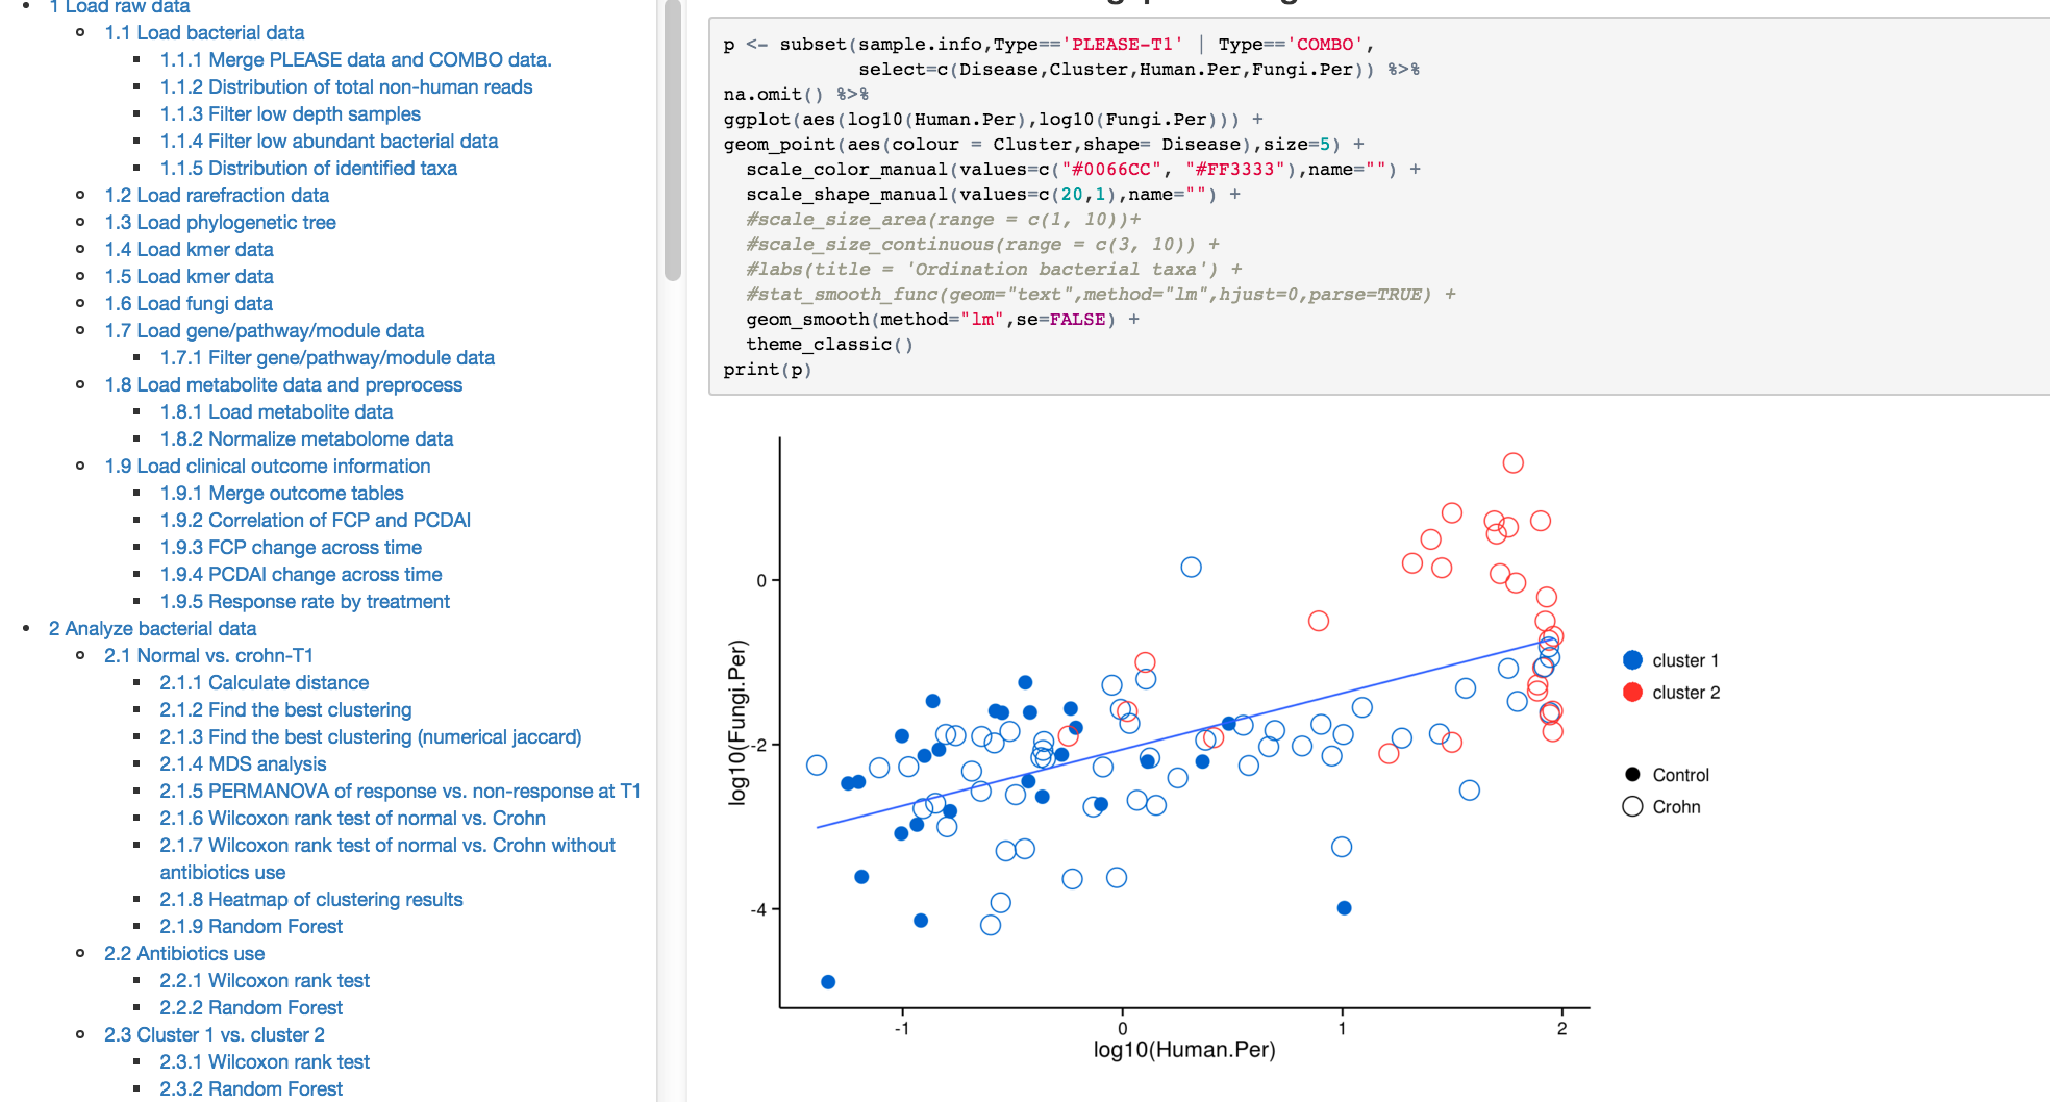
\includegraphics[scale=0.4,trim=0 0 0 0,clip]{Figure/F61_Reproducible_Research.pdf}}
	\caption[An example of RMarkdown report]{An example of Rmarkdown report. The RMarkdown integrates R code, analysis output such as numbers, figures, tables, and annotation text. The analysis in the RMarkdown report is organized and indexed by an index table.  All the analyses included in this dissertation were implemented as RMarkdown reports.
	}
	\label{F61_Reproducible_Research}
\end{figure*}


To make sure that all the statistical models proposed in this dissertation can be easily applied by other researchers in their research, I implemented the statistical models in R packages and made them  available in Github (Figure~\ref{Github_MSSQ}). Github is freely accessible to public users and it is easy to install R package directly from Github. In this way, researchers do not need to implement the proposed statistical models by themselves. Users who identify bugs in the package or have any improvement suggestions can comment on the corresponding  package website. 

\begin{figure*}[p]
	\centering
	{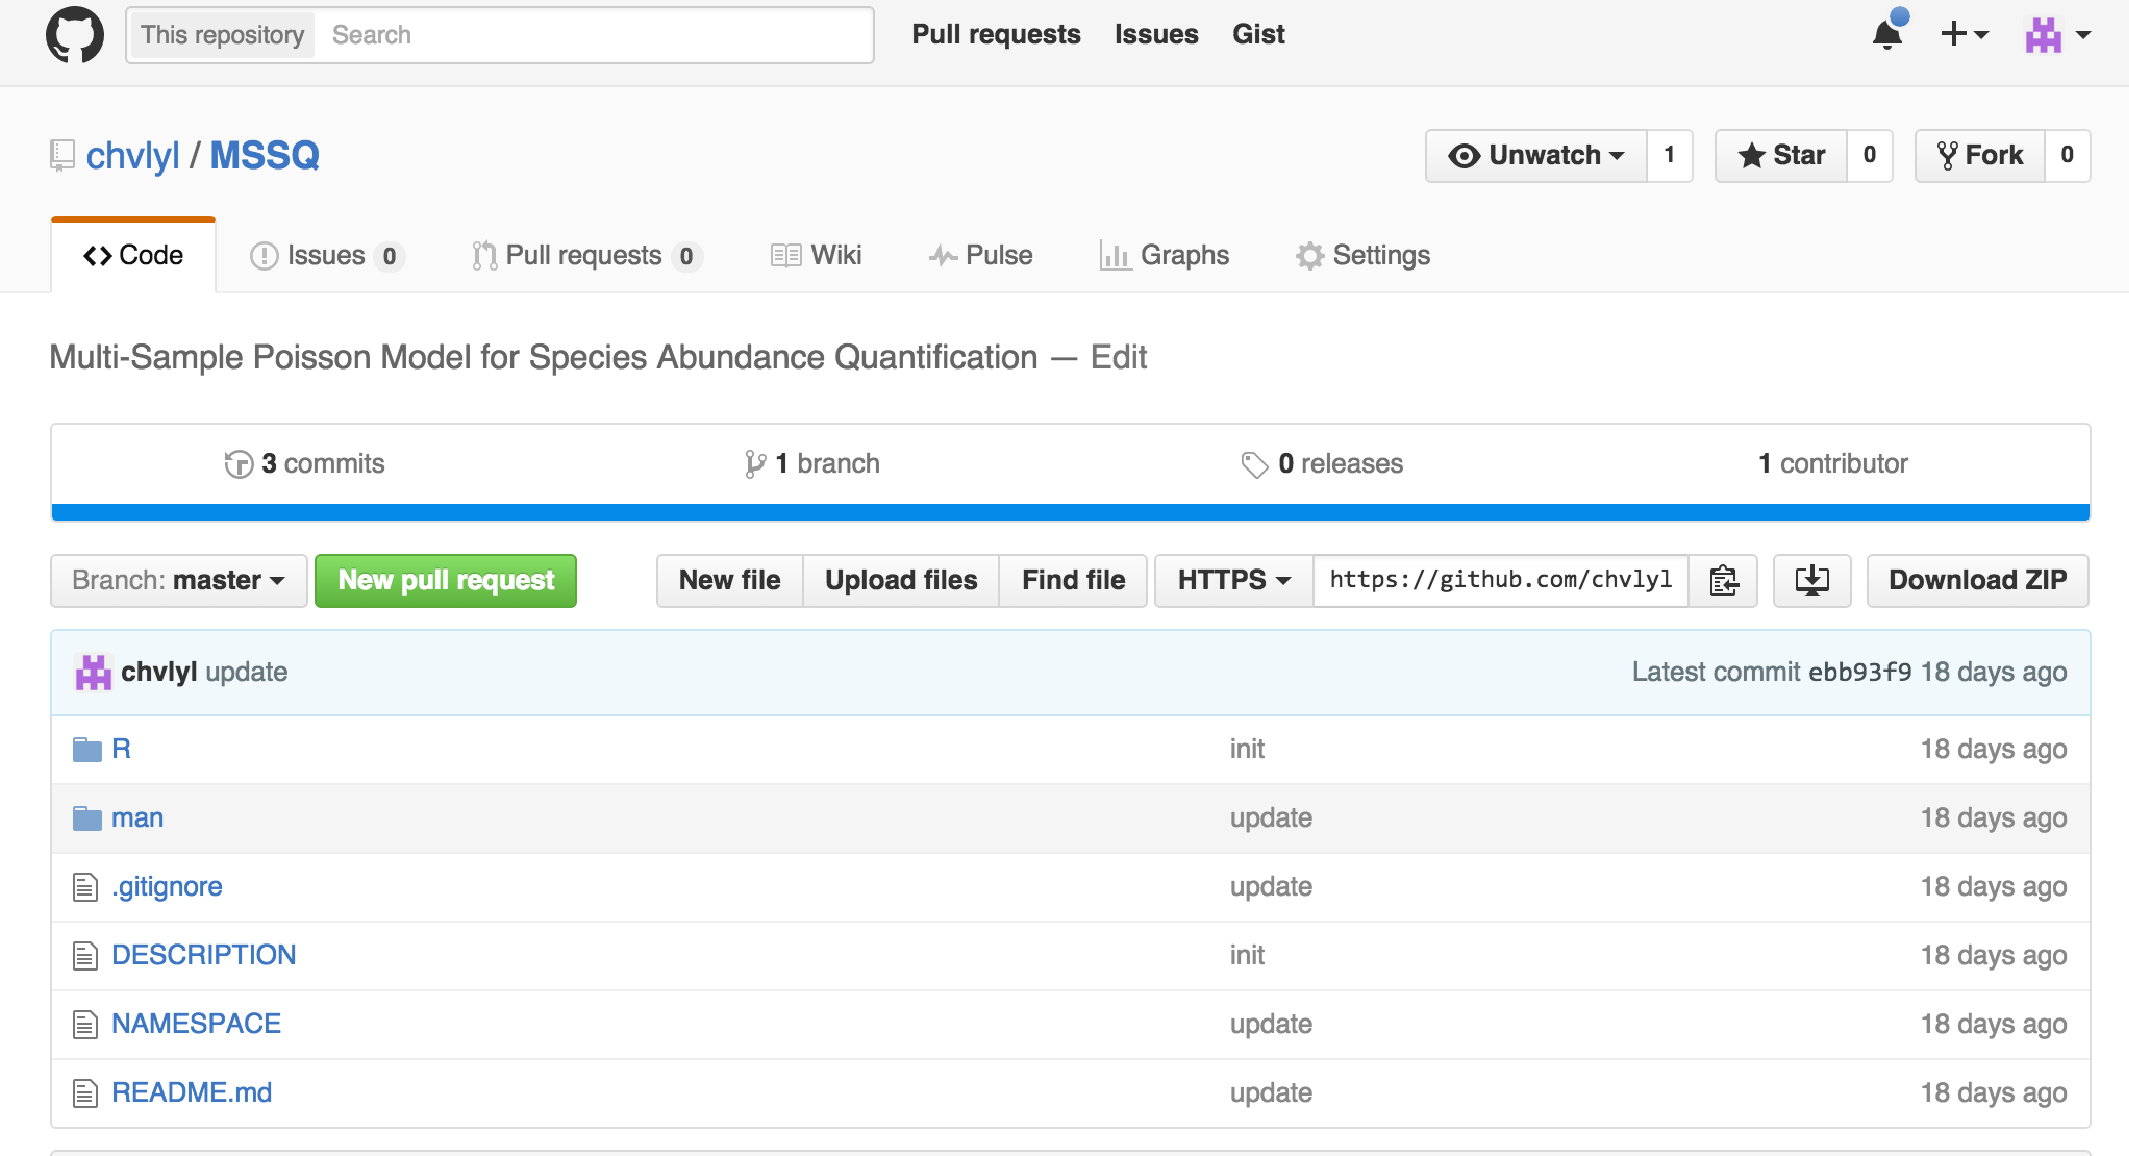
\includegraphics[scale=0.4,trim=0 0 0 0,clip]{Figure/F62_Github_MSSQ1.pdf}
	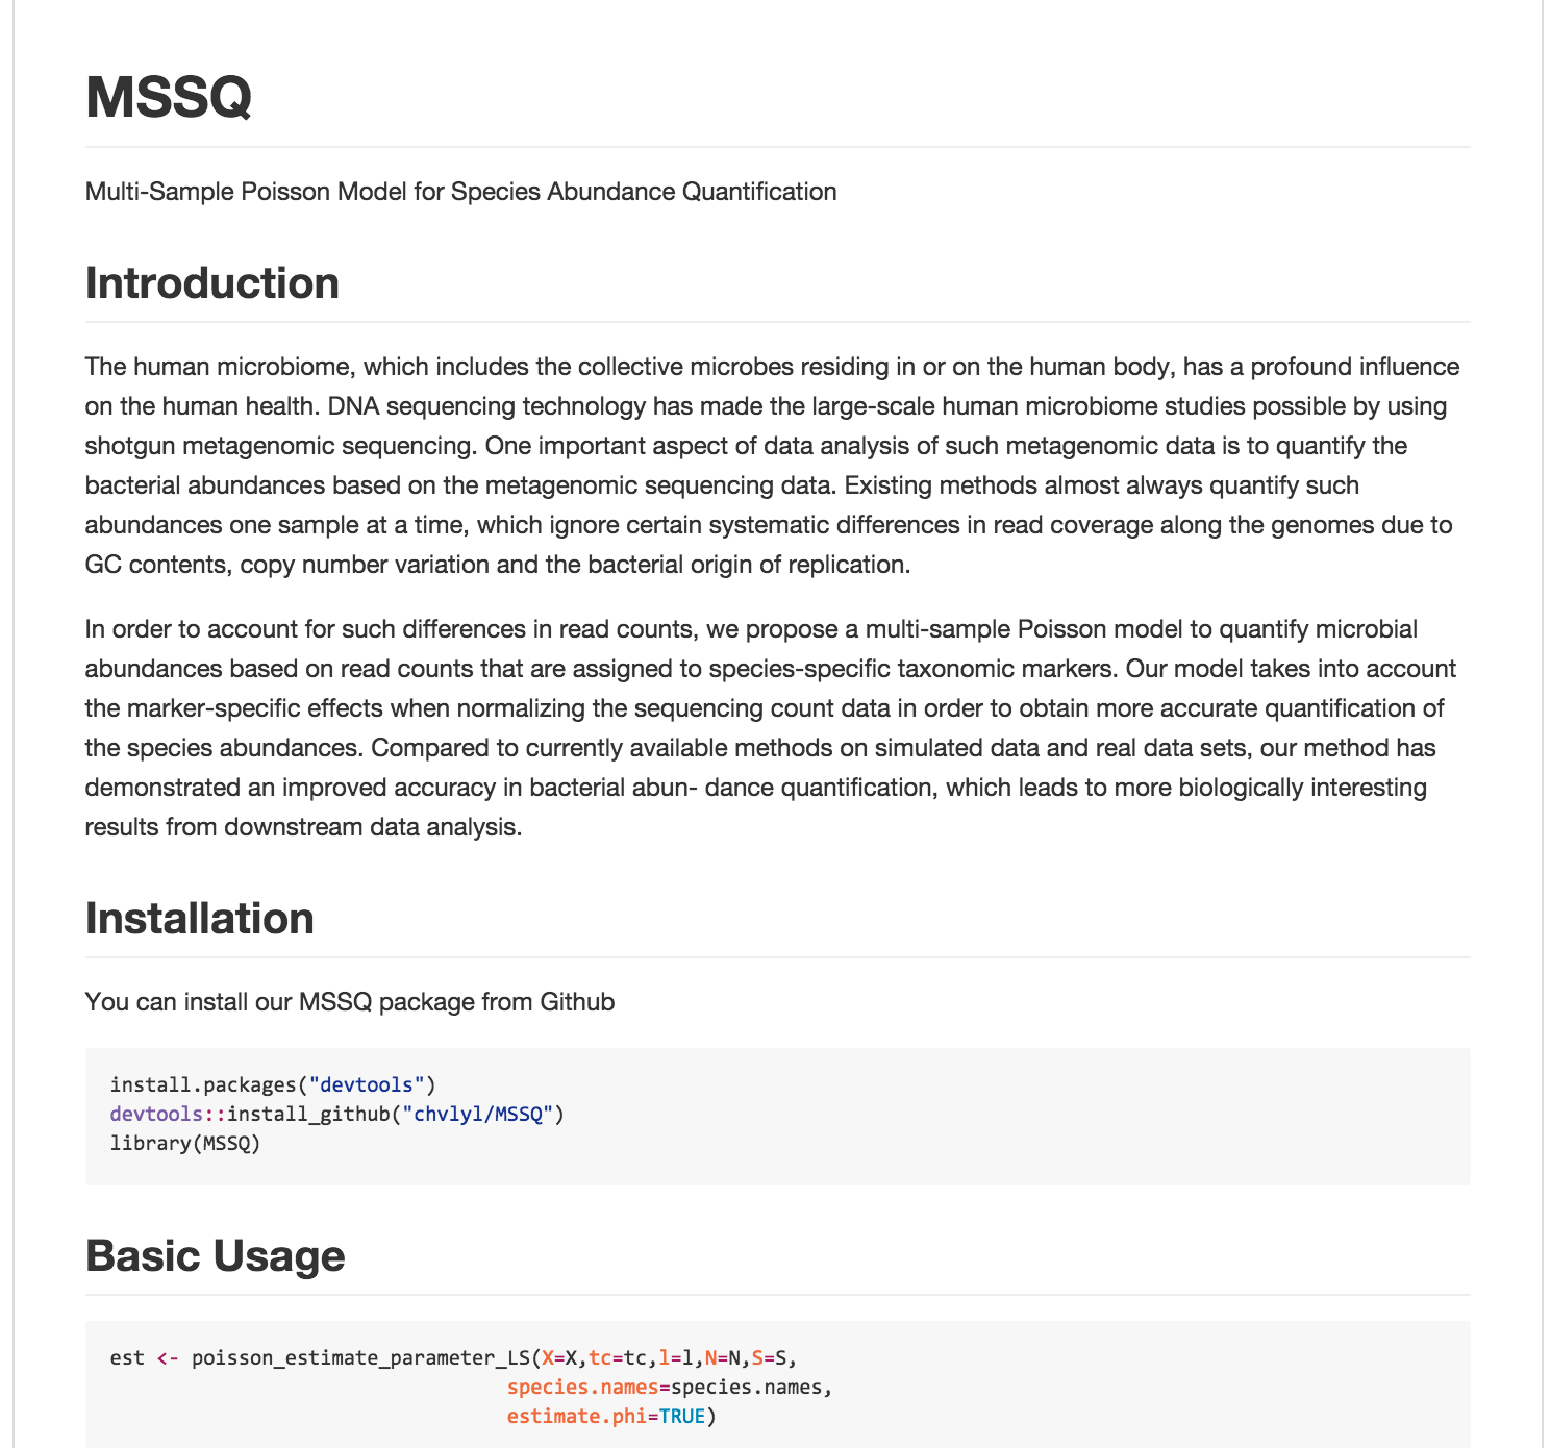
\includegraphics[scale=0.4,trim=0 0 0 0,clip]{Figure/F63_Github_MSSQ2.pdf}
		
	}
	\caption[An example of R packages distributed on Github]{An example of R package MSSQ on Github. Researchers who are interested in using this package can easily install it from Github. All the code are freely available to the public users. An instruction of the package is also included at the main website of this package. Another R package ZIBR introduced in this dissertation was also submitted to Github in a similar fashion.
	}
	\label{Github_MSSQ}
\end{figure*}


Some analyses are also implemented in interactive web applications with R Shiny (Figure~\ref{F64_Shiny}). Users can explore the analyses and results  by simply changing certain parameters. The figures are then  automatically updated. This is especially useful in exploratory statistical analysis that researchers want to investigate  certain  analysis using  different parameter settings.


\begin{figure*}[p]
	\centering
	{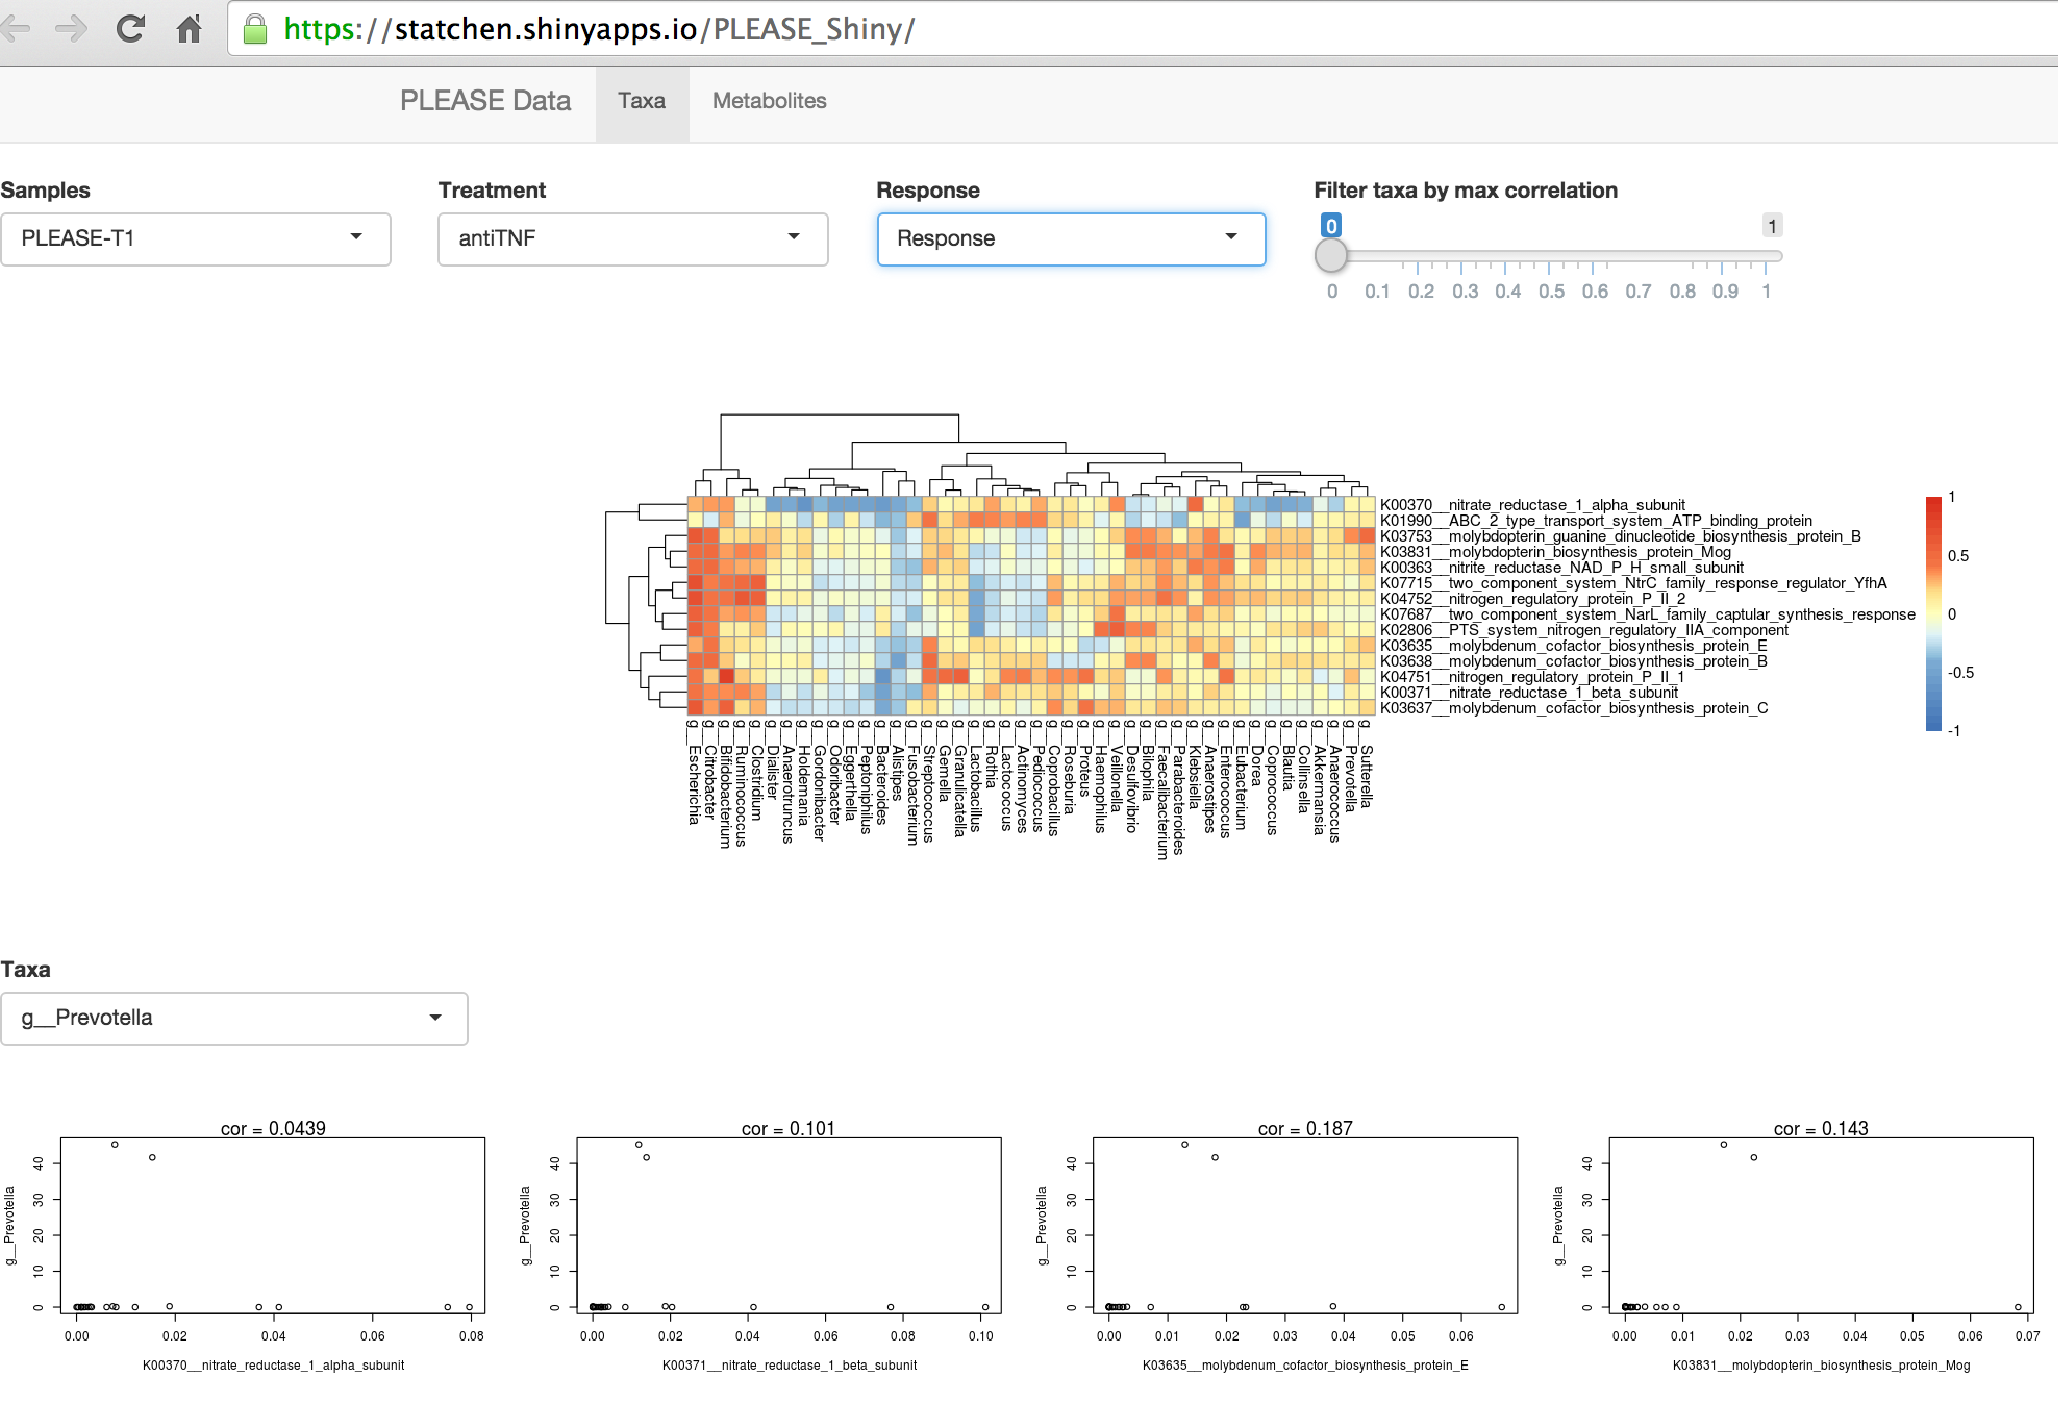
\includegraphics[scale=0.4,trim=0 0 0 0,clip]{Figure/F64_Shiny.pdf}
	}
	\caption[An illustration of interactive analysis of microbiome data]{An illustration of interactive analysis of microbiome data. Users can analyze and visualize the correlations between metabolites and bacterial taxa in different groups. Users  can also filter out the taxa with low correlations. The figure is  automatically updated after users change the setting. This interactive web application was implemented with R Shinny. 
	}
	\label{F64_Shiny}
\end{figure*}